% Created by tikzDevice version 0.8.1 on 2015-11-17 12:44:46
% !TEX encoding = UTF-8 Unicode
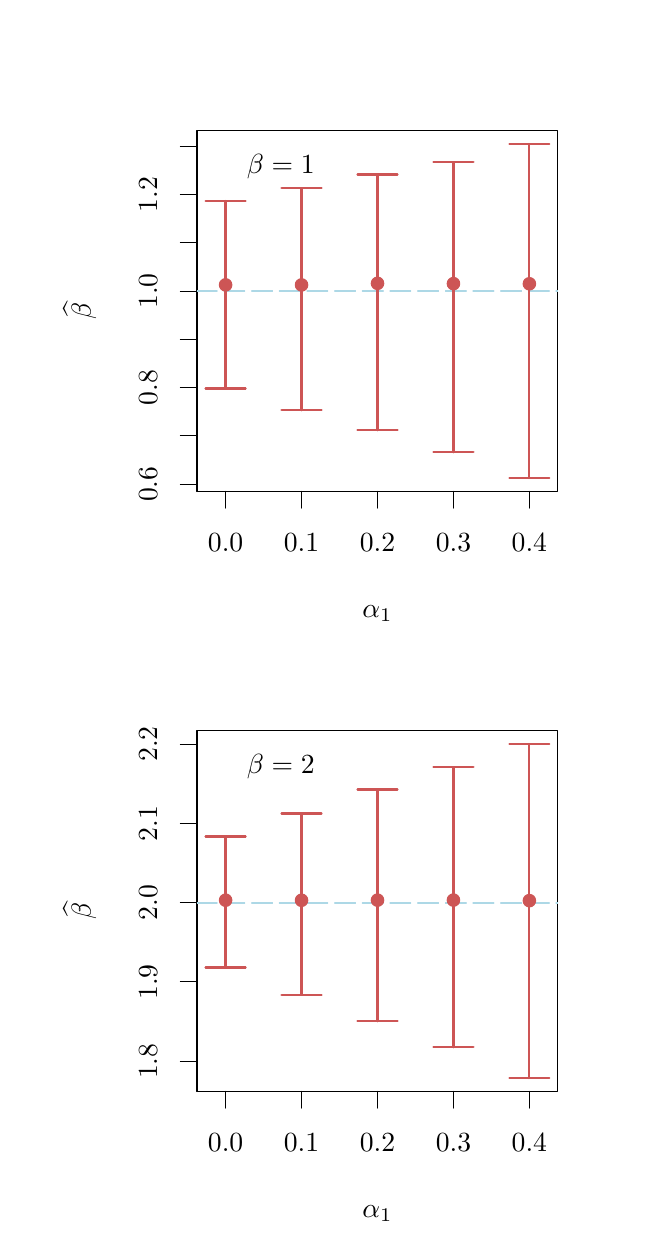
\begin{tikzpicture}[x=1pt,y=1pt]
\definecolor{fillColor}{RGB}{255,255,255}
\path[use as bounding box,fill=fillColor,fill opacity=0.00] (0,0) rectangle (216.81,433.62);
\begin{scope}
\path[clip] ( 61.20,266.01) rectangle (191.61,396.42);
\definecolor{drawColor}{RGB}{255,255,255}
\definecolor{fillColor}{RGB}{255,255,255}

\path[draw=drawColor,line width= 0.4pt,line join=round,line cap=round,fill=fillColor] ( 71.52,340.68) circle (  2.25);

\path[draw=drawColor,line width= 0.4pt,line join=round,line cap=round,fill=fillColor] ( 98.96,340.66) circle (  2.25);

\path[draw=drawColor,line width= 0.4pt,line join=round,line cap=round,fill=fillColor] (126.41,341.23) circle (  2.25);

\path[draw=drawColor,line width= 0.4pt,line join=round,line cap=round,fill=fillColor] (153.85,341.12) circle (  2.25);

\path[draw=drawColor,line width= 0.4pt,line join=round,line cap=round,fill=fillColor] (181.29,341.07) circle (  2.25);
\end{scope}
\begin{scope}
\path[clip] (  0.00,  0.00) rectangle (216.81,433.62);
\definecolor{drawColor}{RGB}{0,0,0}

\path[draw=drawColor,line width= 0.4pt,line join=round,line cap=round] ( 71.52,266.01) -- (181.29,266.01);

\path[draw=drawColor,line width= 0.4pt,line join=round,line cap=round] ( 71.52,266.01) -- ( 71.52,260.01);

\path[draw=drawColor,line width= 0.4pt,line join=round,line cap=round] ( 98.96,266.01) -- ( 98.96,260.01);

\path[draw=drawColor,line width= 0.4pt,line join=round,line cap=round] (126.41,266.01) -- (126.41,260.01);

\path[draw=drawColor,line width= 0.4pt,line join=round,line cap=round] (153.85,266.01) -- (153.85,260.01);

\path[draw=drawColor,line width= 0.4pt,line join=round,line cap=round] (181.29,266.01) -- (181.29,260.01);

\node[text=drawColor,anchor=base,inner sep=0pt, outer sep=0pt, scale=  1.00] at ( 71.52,244.41) {0.0};

\node[text=drawColor,anchor=base,inner sep=0pt, outer sep=0pt, scale=  1.00] at ( 98.96,244.41) {0.1};

\node[text=drawColor,anchor=base,inner sep=0pt, outer sep=0pt, scale=  1.00] at (126.41,244.41) {0.2};

\node[text=drawColor,anchor=base,inner sep=0pt, outer sep=0pt, scale=  1.00] at (153.85,244.41) {0.3};

\node[text=drawColor,anchor=base,inner sep=0pt, outer sep=0pt, scale=  1.00] at (181.29,244.41) {0.4};

\path[draw=drawColor,line width= 0.4pt,line join=round,line cap=round] ( 61.20,268.63) -- ( 61.20,390.80);

\path[draw=drawColor,line width= 0.4pt,line join=round,line cap=round] ( 61.20,268.63) -- ( 55.20,268.63);

\path[draw=drawColor,line width= 0.4pt,line join=round,line cap=round] ( 61.20,286.09) -- ( 55.20,286.09);

\path[draw=drawColor,line width= 0.4pt,line join=round,line cap=round] ( 61.20,303.54) -- ( 55.20,303.54);

\path[draw=drawColor,line width= 0.4pt,line join=round,line cap=round] ( 61.20,320.99) -- ( 55.20,320.99);

\path[draw=drawColor,line width= 0.4pt,line join=round,line cap=round] ( 61.20,338.44) -- ( 55.20,338.44);

\path[draw=drawColor,line width= 0.4pt,line join=round,line cap=round] ( 61.20,355.90) -- ( 55.20,355.90);

\path[draw=drawColor,line width= 0.4pt,line join=round,line cap=round] ( 61.20,373.35) -- ( 55.20,373.35);

\path[draw=drawColor,line width= 0.4pt,line join=round,line cap=round] ( 61.20,390.80) -- ( 55.20,390.80);

\node[text=drawColor,rotate= 90.00,anchor=base,inner sep=0pt, outer sep=0pt, scale=  1.00] at ( 46.80,268.63) {0.6};

\node[text=drawColor,rotate= 90.00,anchor=base,inner sep=0pt, outer sep=0pt, scale=  1.00] at ( 46.80,303.54) {0.8};

\node[text=drawColor,rotate= 90.00,anchor=base,inner sep=0pt, outer sep=0pt, scale=  1.00] at ( 46.80,338.44) {1.0};

\node[text=drawColor,rotate= 90.00,anchor=base,inner sep=0pt, outer sep=0pt, scale=  1.00] at ( 46.80,373.35) {1.2};

\path[draw=drawColor,line width= 0.4pt,line join=round,line cap=round] ( 61.20,266.01) --
	(191.61,266.01) --
	(191.61,396.42) --
	( 61.20,396.42) --
	( 61.20,266.01);
\end{scope}
\begin{scope}
\path[clip] (  0.00,216.81) rectangle (216.81,433.62);
\definecolor{drawColor}{RGB}{0,0,0}

\node[text=drawColor,anchor=base,inner sep=0pt, outer sep=0pt, scale=  1.00] at (126.41,220.41) {$\alpha_1$};

\node[text=drawColor,rotate= 90.00,anchor=base,inner sep=0pt, outer sep=0pt, scale=  1.00] at ( 22.80,331.22) {$\widehat{\beta}$};
\end{scope}
\begin{scope}
\path[clip] ( 61.20,266.01) rectangle (191.61,396.42);
\definecolor{drawColor}{RGB}{0,0,0}

\node[text=drawColor,anchor=base west,inner sep=0pt, outer sep=0pt, scale=  1.00] at ( 79.20,380.98) {$\beta=1$};
\definecolor{drawColor}{RGB}{173,216,230}

\path[draw=drawColor,line width= 0.8pt,dash pattern=on 7pt off 3pt ,line join=round,line cap=round] ( 61.20,338.44) -- (191.61,338.44);

\path[draw=drawColor,line width= 0.8pt,dash pattern=on 7pt off 3pt ,line join=round,line cap=round] ( 61.20,338.44) -- (191.61,338.44);

\path[draw=drawColor,line width= 0.8pt,dash pattern=on 7pt off 3pt ,line join=round,line cap=round] ( 61.20,338.44) -- (191.61,338.44);

\path[draw=drawColor,line width= 0.8pt,dash pattern=on 7pt off 3pt ,line join=round,line cap=round] ( 61.20,338.44) -- (191.61,338.44);

\path[draw=drawColor,line width= 0.8pt,dash pattern=on 7pt off 3pt ,line join=round,line cap=round] ( 61.20,338.44) -- (191.61,338.44);
\definecolor{drawColor}{RGB}{205,85,85}

\path[draw=drawColor,line width= 0.8pt,line join=round,line cap=round] ( 71.52,303.21) -- ( 71.52,370.97);

\path[draw=drawColor,line width= 0.8pt,line join=round,line cap=round] ( 64.29,303.21) --
	( 71.52,303.21) --
	( 78.75,303.21);

\path[draw=drawColor,line width= 0.8pt,line join=round,line cap=round] ( 78.75,370.97) --
	( 71.52,370.97) --
	( 64.29,370.97);

\path[draw=drawColor,line width= 0.8pt,line join=round,line cap=round] ( 98.96,295.39) -- ( 98.96,375.63);

\path[draw=drawColor,line width= 0.8pt,line join=round,line cap=round] ( 91.73,295.39) --
	( 98.96,295.39) --
	(106.19,295.39);

\path[draw=drawColor,line width= 0.8pt,line join=round,line cap=round] (106.19,375.63) --
	( 98.96,375.63) --
	( 91.73,375.63);

\path[draw=drawColor,line width= 0.8pt,line join=round,line cap=round] (126.41,288.16) -- (126.41,380.54);

\path[draw=drawColor,line width= 0.8pt,line join=round,line cap=round] (119.18,288.16) --
	(126.41,288.16) --
	(133.63,288.16);

\path[draw=drawColor,line width= 0.8pt,line join=round,line cap=round] (133.63,380.54) --
	(126.41,380.54) --
	(119.18,380.54);

\path[draw=drawColor,line width= 0.8pt,line join=round,line cap=round] (153.85,280.22) -- (153.85,384.97);

\path[draw=drawColor,line width= 0.8pt,line join=round,line cap=round] (146.62,280.22) --
	(153.85,280.22) --
	(161.08,280.22);

\path[draw=drawColor,line width= 0.8pt,line join=round,line cap=round] (161.08,384.97) --
	(153.85,384.97) --
	(146.62,384.97);

\path[draw=drawColor,line width= 0.8pt,line join=round,line cap=round] (181.29,270.84) -- (181.29,391.59);

\path[draw=drawColor,line width= 0.8pt,line join=round,line cap=round] (174.06,270.84) --
	(181.29,270.84) --
	(188.52,270.84);

\path[draw=drawColor,line width= 0.8pt,line join=round,line cap=round] (188.52,391.59) --
	(181.29,391.59) --
	(174.06,391.59);
\definecolor{fillColor}{RGB}{205,85,85}

\path[draw=drawColor,line width= 0.4pt,line join=round,line cap=round,fill=fillColor] ( 71.52,340.68) circle (  2.25);

\path[draw=drawColor,line width= 0.4pt,line join=round,line cap=round,fill=fillColor] ( 98.96,340.66) circle (  2.25);

\path[draw=drawColor,line width= 0.4pt,line join=round,line cap=round,fill=fillColor] (126.41,341.23) circle (  2.25);

\path[draw=drawColor,line width= 0.4pt,line join=round,line cap=round,fill=fillColor] (153.85,341.12) circle (  2.25);

\path[draw=drawColor,line width= 0.4pt,line join=round,line cap=round,fill=fillColor] (181.29,341.07) circle (  2.25);
\end{scope}
\begin{scope}
\path[clip] ( 61.20, 49.20) rectangle (191.61,179.61);
\definecolor{drawColor}{RGB}{255,255,255}
\definecolor{fillColor}{RGB}{255,255,255}

\path[draw=drawColor,line width= 0.4pt,line join=round,line cap=round,fill=fillColor] ( 71.52,118.33) circle (  2.25);

\path[draw=drawColor,line width= 0.4pt,line join=round,line cap=round,fill=fillColor] ( 98.96,118.30) circle (  2.25);

\path[draw=drawColor,line width= 0.4pt,line join=round,line cap=round,fill=fillColor] (126.41,118.35) circle (  2.25);

\path[draw=drawColor,line width= 0.4pt,line join=round,line cap=round,fill=fillColor] (153.85,118.37) circle (  2.25);

\path[draw=drawColor,line width= 0.4pt,line join=round,line cap=round,fill=fillColor] (181.29,118.17) circle (  2.25);
\end{scope}
\begin{scope}
\path[clip] (  0.00,  0.00) rectangle (216.81,433.62);
\definecolor{drawColor}{RGB}{0,0,0}

\path[draw=drawColor,line width= 0.4pt,line join=round,line cap=round] ( 71.52, 49.20) -- (181.29, 49.20);

\path[draw=drawColor,line width= 0.4pt,line join=round,line cap=round] ( 71.52, 49.20) -- ( 71.52, 43.20);

\path[draw=drawColor,line width= 0.4pt,line join=round,line cap=round] ( 98.96, 49.20) -- ( 98.96, 43.20);

\path[draw=drawColor,line width= 0.4pt,line join=round,line cap=round] (126.41, 49.20) -- (126.41, 43.20);

\path[draw=drawColor,line width= 0.4pt,line join=round,line cap=round] (153.85, 49.20) -- (153.85, 43.20);

\path[draw=drawColor,line width= 0.4pt,line join=round,line cap=round] (181.29, 49.20) -- (181.29, 43.20);

\node[text=drawColor,anchor=base,inner sep=0pt, outer sep=0pt, scale=  1.00] at ( 71.52, 27.60) {0.0};

\node[text=drawColor,anchor=base,inner sep=0pt, outer sep=0pt, scale=  1.00] at ( 98.96, 27.60) {0.1};

\node[text=drawColor,anchor=base,inner sep=0pt, outer sep=0pt, scale=  1.00] at (126.41, 27.60) {0.2};

\node[text=drawColor,anchor=base,inner sep=0pt, outer sep=0pt, scale=  1.00] at (153.85, 27.60) {0.3};

\node[text=drawColor,anchor=base,inner sep=0pt, outer sep=0pt, scale=  1.00] at (181.29, 27.60) {0.4};

\path[draw=drawColor,line width= 0.4pt,line join=round,line cap=round] ( 61.20, 60.16) -- ( 61.20,174.72);

\path[draw=drawColor,line width= 0.4pt,line join=round,line cap=round] ( 61.20, 60.16) -- ( 55.20, 60.16);

\path[draw=drawColor,line width= 0.4pt,line join=round,line cap=round] ( 61.20, 88.80) -- ( 55.20, 88.80);

\path[draw=drawColor,line width= 0.4pt,line join=round,line cap=round] ( 61.20,117.44) -- ( 55.20,117.44);

\path[draw=drawColor,line width= 0.4pt,line join=round,line cap=round] ( 61.20,146.08) -- ( 55.20,146.08);

\path[draw=drawColor,line width= 0.4pt,line join=round,line cap=round] ( 61.20,174.72) -- ( 55.20,174.72);

\node[text=drawColor,rotate= 90.00,anchor=base,inner sep=0pt, outer sep=0pt, scale=  1.00] at ( 46.80, 60.16) {1.8};

\node[text=drawColor,rotate= 90.00,anchor=base,inner sep=0pt, outer sep=0pt, scale=  1.00] at ( 46.80, 88.80) {1.9};

\node[text=drawColor,rotate= 90.00,anchor=base,inner sep=0pt, outer sep=0pt, scale=  1.00] at ( 46.80,117.44) {2.0};

\node[text=drawColor,rotate= 90.00,anchor=base,inner sep=0pt, outer sep=0pt, scale=  1.00] at ( 46.80,146.08) {2.1};

\node[text=drawColor,rotate= 90.00,anchor=base,inner sep=0pt, outer sep=0pt, scale=  1.00] at ( 46.80,174.72) {2.2};

\path[draw=drawColor,line width= 0.4pt,line join=round,line cap=round] ( 61.20, 49.20) --
	(191.61, 49.20) --
	(191.61,179.61) --
	( 61.20,179.61) --
	( 61.20, 49.20);
\end{scope}
\begin{scope}
\path[clip] (  0.00,  0.00) rectangle (216.81,216.81);
\definecolor{drawColor}{RGB}{0,0,0}

\node[text=drawColor,anchor=base,inner sep=0pt, outer sep=0pt, scale=  1.00] at (126.41,  3.60) {$\alpha_1$};

\node[text=drawColor,rotate= 90.00,anchor=base,inner sep=0pt, outer sep=0pt, scale=  1.00] at ( 22.80,114.41) {$\widehat{\beta}$};
\end{scope}
\begin{scope}
\path[clip] ( 61.20, 49.20) rectangle (191.61,179.61);
\definecolor{drawColor}{RGB}{0,0,0}

\node[text=drawColor,anchor=base west,inner sep=0pt, outer sep=0pt, scale=  1.00] at ( 79.20,164.17) {$\beta=2$};
\definecolor{drawColor}{RGB}{173,216,230}

\path[draw=drawColor,line width= 0.8pt,dash pattern=on 7pt off 3pt ,line join=round,line cap=round] ( 61.20,117.44) -- (191.61,117.44);

\path[draw=drawColor,line width= 0.8pt,dash pattern=on 7pt off 3pt ,line join=round,line cap=round] ( 61.20,117.44) -- (191.61,117.44);

\path[draw=drawColor,line width= 0.8pt,dash pattern=on 7pt off 3pt ,line join=round,line cap=round] ( 61.20,117.44) -- (191.61,117.44);

\path[draw=drawColor,line width= 0.8pt,dash pattern=on 7pt off 3pt ,line join=round,line cap=round] ( 61.20,117.44) -- (191.61,117.44);

\path[draw=drawColor,line width= 0.8pt,dash pattern=on 7pt off 3pt ,line join=round,line cap=round] ( 61.20,117.44) -- (191.61,117.44);
\definecolor{drawColor}{RGB}{205,85,85}

\path[draw=drawColor,line width= 0.8pt,line join=round,line cap=round] ( 71.52, 94.03) -- ( 71.52,141.36);

\path[draw=drawColor,line width= 0.8pt,line join=round,line cap=round] ( 64.29, 94.03) --
	( 71.52, 94.03) --
	( 78.75, 94.03);

\path[draw=drawColor,line width= 0.8pt,line join=round,line cap=round] ( 78.75,141.36) --
	( 71.52,141.36) --
	( 64.29,141.36);

\path[draw=drawColor,line width= 0.8pt,line join=round,line cap=round] ( 98.96, 84.20) -- ( 98.96,149.64);

\path[draw=drawColor,line width= 0.8pt,line join=round,line cap=round] ( 91.73, 84.20) --
	( 98.96, 84.20) --
	(106.19, 84.20);

\path[draw=drawColor,line width= 0.8pt,line join=round,line cap=round] (106.19,149.64) --
	( 98.96,149.64) --
	( 91.73,149.64);

\path[draw=drawColor,line width= 0.8pt,line join=round,line cap=round] (126.41, 74.61) -- (126.41,158.31);

\path[draw=drawColor,line width= 0.8pt,line join=round,line cap=round] (119.18, 74.61) --
	(126.41, 74.61) --
	(133.63, 74.61);

\path[draw=drawColor,line width= 0.8pt,line join=round,line cap=round] (133.63,158.31) --
	(126.41,158.31) --
	(119.18,158.31);

\path[draw=drawColor,line width= 0.8pt,line join=round,line cap=round] (153.85, 65.20) -- (153.85,166.39);

\path[draw=drawColor,line width= 0.8pt,line join=round,line cap=round] (146.62, 65.20) --
	(153.85, 65.20) --
	(161.08, 65.20);

\path[draw=drawColor,line width= 0.8pt,line join=round,line cap=round] (161.08,166.39) --
	(153.85,166.39) --
	(146.62,166.39);

\path[draw=drawColor,line width= 0.8pt,line join=round,line cap=round] (181.29, 54.03) -- (181.29,174.78);

\path[draw=drawColor,line width= 0.8pt,line join=round,line cap=round] (174.06, 54.03) --
	(181.29, 54.03) --
	(188.52, 54.03);

\path[draw=drawColor,line width= 0.8pt,line join=round,line cap=round] (188.52,174.78) --
	(181.29,174.78) --
	(174.06,174.78);
\definecolor{fillColor}{RGB}{205,85,85}

\path[draw=drawColor,line width= 0.4pt,line join=round,line cap=round,fill=fillColor] ( 71.52,118.33) circle (  2.25);

\path[draw=drawColor,line width= 0.4pt,line join=round,line cap=round,fill=fillColor] ( 98.96,118.30) circle (  2.25);

\path[draw=drawColor,line width= 0.4pt,line join=round,line cap=round,fill=fillColor] (126.41,118.35) circle (  2.25);

\path[draw=drawColor,line width= 0.4pt,line join=round,line cap=round,fill=fillColor] (153.85,118.37) circle (  2.25);

\path[draw=drawColor,line width= 0.4pt,line join=round,line cap=round,fill=fillColor] (181.29,118.17) circle (  2.25);
\end{scope}
\end{tikzpicture}
